\documentclass[a4paper,12pt,notitlepage]{amsart}
\usepackage{amsfonts, amsmath, amscd, amsthm, graphicx, amssymb}
\usepackage{tikz}
\usepackage{tikz-cd}

\begin{document}

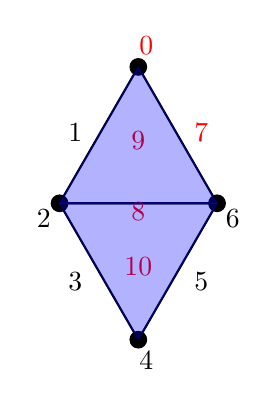
\begin{tikzpicture}
			%% vertices
			\draw[fill=black] (0,1.732) circle (3pt);
			\draw[fill=black] (1,0) circle (3pt);
			\draw[fill=black] (-1,0) circle (3pt);
			\draw[fill=black] (0,-1.732) circle (3pt);
			%% vertex labels
			%%% edges
			\draw[thick] (1,0) -- (-1,0) -- (0,1.732)-- (1,0);
			\draw[thick] (1,0) -- (-1,0) -- (0,-1.732)-- (1,0);			
			
			
			
			\node[red] at (0,-0.1) {$8$};			
			\node at (-0.8,0.9) {$1$};
			\node[red] at (0.8,0.9) {$7$};
			
			
			\node at (1.2,-0.2) {$6$};			
			\node at (-1.2,-0.2) {$2$};
			\node[red] at (0.1,2) {$0$};
			
			
			\node at (0.1,-2) {$4$};
			\node at (-0.8,-1.0) {$3$};
			\node at (0.8,-1.0) {$5$};			
			
			\node[red] at (0,0.8) {$9$};	
			\node[red] at (0,-0.8) {$10$};		
			
			\filldraw[opacity=.3, blue] (1,0) -- (-1,0) -- (0,1.732)-- (1,0);
			\filldraw[opacity=.3, blue] (1,0) -- (-1,0) -- (0,-1.732)-- (1,0);
			

		\end{tikzpicture}

\end{document}